% HET FTS

As discussed in the previous section, successful modeling of the
iodine observations (B star spectra taken through the Iodien cell) is
a good indication of a working radial velocity (RV) pipeline. At
Keck/HIRES, which has demosntrated 1 m/s RV precision over the years,
the modeling of the iodine observations yields a reduced chi-square
(\chisq) value of typically 1.05. However, for HET/HRS iodine
observations, with the same RV pipeline used at Keck, the typical
\chisq\ value is $>2$ or even $>5$ for some observations. 

We have explored one of the two model components for modeling iodine
observations, the choice of IP. In this section, we examine the other
model component, the iodine atlas, that is, the ``ground truth''
spectrum for the iodine absorption lines unique to the \het\ iodine
cell. We came upon an interesting lead which made us believe that
there might have been changes in the iodine cell itself and its
enclosure.


%%%%%%%%%%%%%%%%%%%%%%%%%%%%%%%%%%%%%%%%%%%%%%%%%%%%%%%%%%%%%%%%%%%%%%%%%%%%%%
\subsection{Motivation}

As we were investigating the reasons behind the apparent `bad fit' of
\het\ iodine observations, we decided to check the quality of the
existing iodine atlas. An iodine atlas is normally obtained using a
Fourier Transform Spectrometer (FTS; whose mechanism is just like a
Michelson interferometer). The scan and its subsequent data reduction
provides very high resolution spectrum (translated from Fourier space
into real space) with typically $R > 250,000$-500,000.\footnote{It is worth
noting here that although FTS normally provides wavelength solutions
(from the registered arm lengths), but because of the inaccuracy of
the default reported wavelengths, the final wavelength solution for
the iodine atlas is usually derived from a theoretically computed iodine
line list (e.g., \citealt{iodinespec5}).}

The existing iodine atlas for the \het\ cell is from an FTS scan taken
at the National Solar Observatory at KPNO using the Babar FTS
(nicknamed for its large size; this machine has been decommissioned)
in 1993. The main reason is that the FTS scan was taken almost two
decades ago, and during this time the cell may have gone through
changes (such as temperature, leaking or condensation, etc., though
unlikely, since the cell was designed to be stable). This would mean
that the FTS scan is out of date and inaccurate, and it could explain
the `bad fits' to the iodine observation.

We therefore took the HET/HRS cell to the National Institute of
Standards and Technology (NIST) and obtained a new FTS scan in 2011
(an effort carried out by Jason Wright, Ming Zhao, Stephen Redman and
others at NIST; data reduction done by Stephen Redman). A close
comparison between this new scan from NIST and the old scan at KPNO
reveals that they have many differences:
\begin{itemize}
  \item The overall line depths are very different --- the NIST scan
    has deeper lines.
  \item The absolute wavelength solutions are different, and the
    drifting of wavelength solution or the dispersion scales at
    different wavelength are also different.
  \item Even after we adjust the `normalization' level of the NIST
    scan (assuming the FTS data has normalization issues or low
    frequency noise/offset), the line ratios of the two scans still
    exhibits differences.
\end{itemize}

Figure~\ref{fig:fts_old_new} shows the comparison between the two
scans in a selected 2\AA\ region. As the two scans also differ in
resolution (the NIST scan has a higher resolution), the middle panel
is a more direct comparison: the NIST scan has been convolved down to
the same resolution with the KPNO scan; it is also shifted in
wavelength space so that the two scans match in absolute wavelength
solution; and it is adjusted to a different ``normalization'' level to
match with the KPNO scan as much as possible in order to compare their
relative line ratios.

    
%----------------------------------------------------------------
% Figure: HET FTS, KPNO old scan vs. NIST new scan
\begin{figure}[!th]
\centering
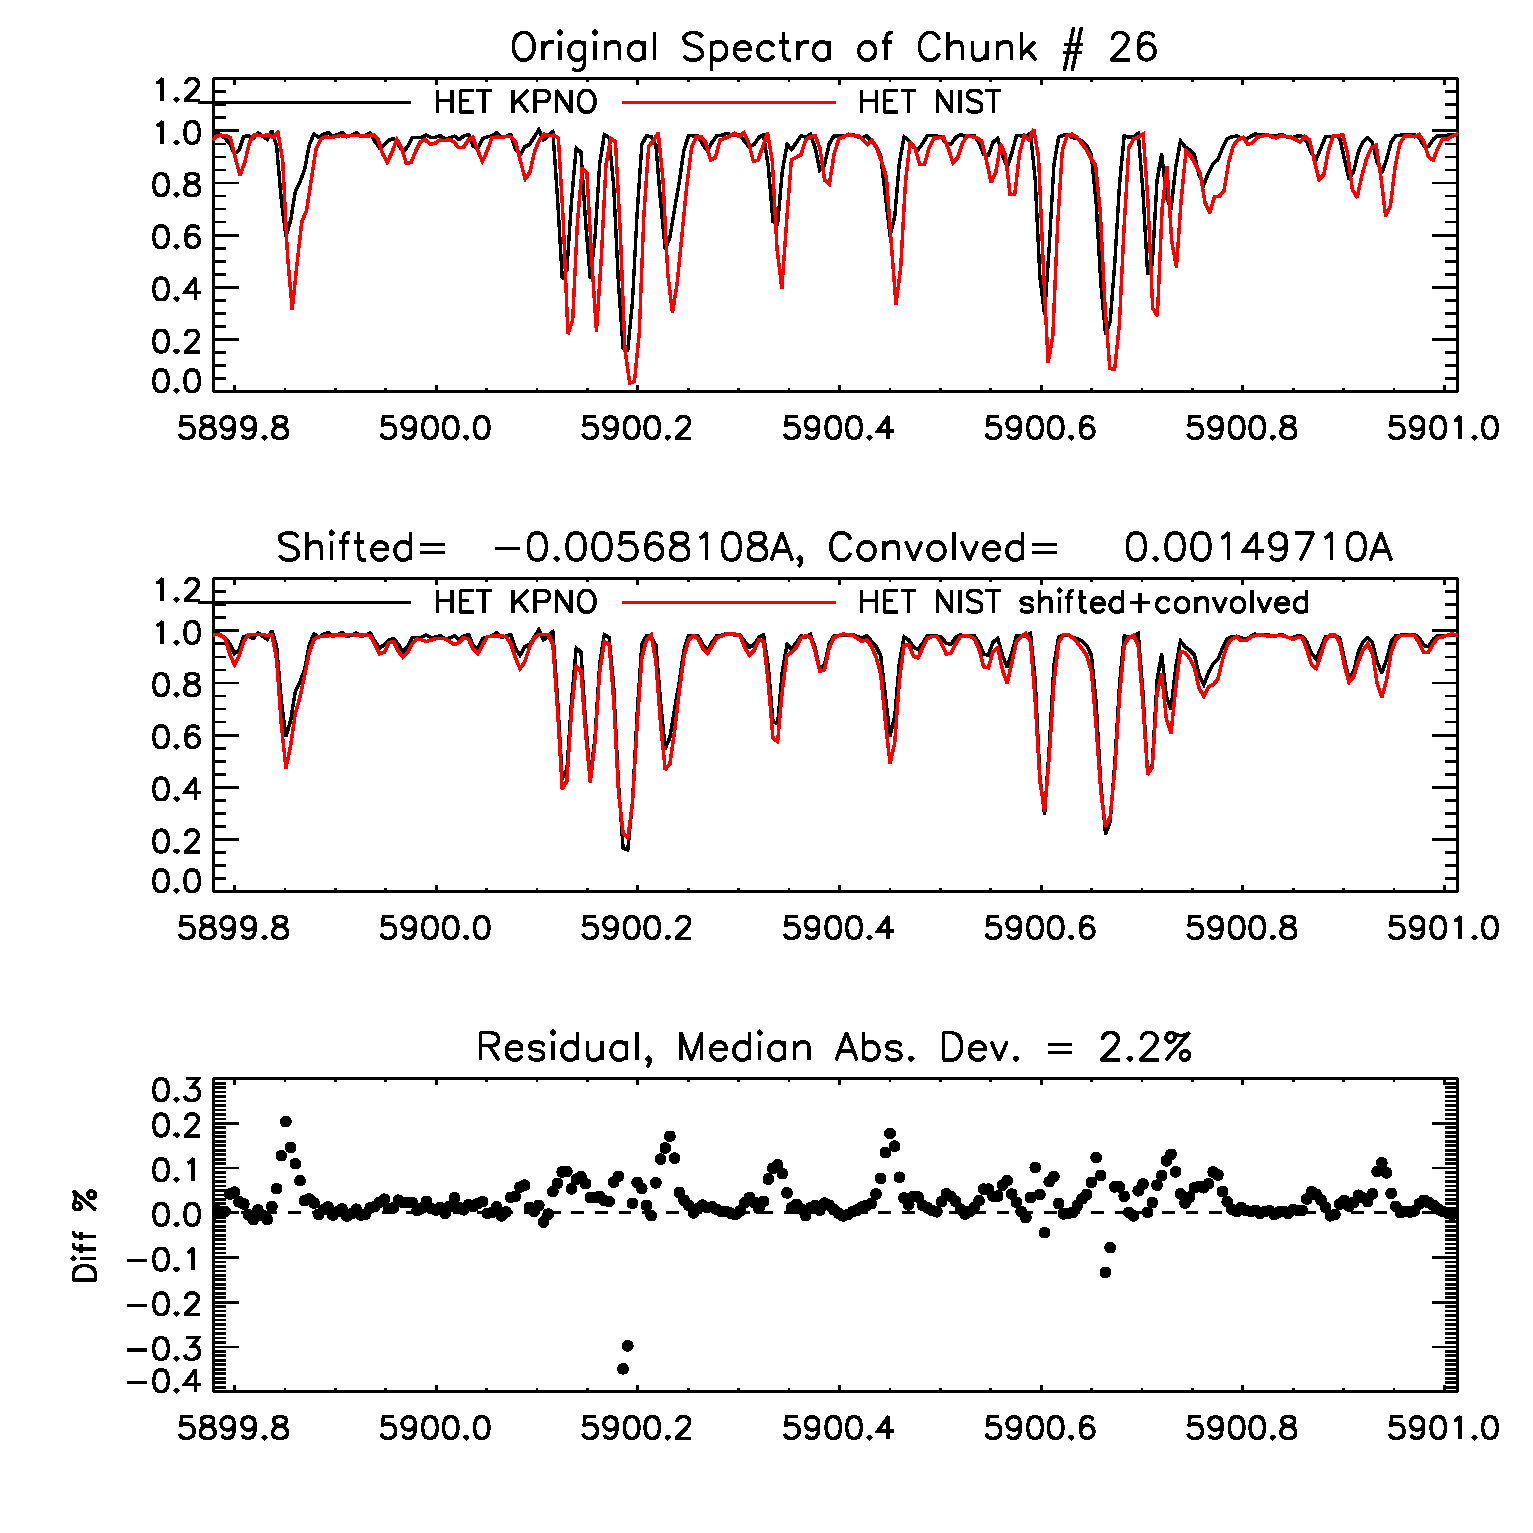
\includegraphics[angle=0.,scale=0.45]{het/compare_het_fts_26.eps}
\caption{Comparison of the KPNO FTS scan (black) and the NIST FTS scan
  (red) for the HET/HRS iodine cell for a selected
  1.5\AA\ chunk. \textbf{Top:} Two scans at their native resolution
  and original wavelength solution. \textbf{Middle:} Comparison of the
  two scans after adjusting the normalization, shifting, and
  convolution for the NIST scan to match the KPNO scan for a more
  direct comparison of line depths/ratios. \textbf{Bottom:} Residuals
  of the middle panel, NIST spectrum minus the KPNO spectrum. The
  median absolute deviation between the two spectra is 0.02
  (2\%), though at many places, especially at line centers, the two
  can differ by up to 5--10\%.
  \label{fig:fts_old_new}}
\end{figure}
%----------------------------------------------------------------

We initially suspected that the NIST scan was problematic. The reason is
illustrated in the left panel of Figure~\ref{fig:chisq_old_new}, where
it shows the histogram of \chisq\ values for fitting an selected iodine
observation using the two scans, respectively. Each \chisq\ value is
for a 2\AA\ chunk in this selected iodine observation. It is clear
that the NIST scan provides worse fits.

%----------------------------------------------------------------
% Figure: chisq of iodine observation fit, KPNO old scan vs. NIST new scan
\begin{figure*}[!th]
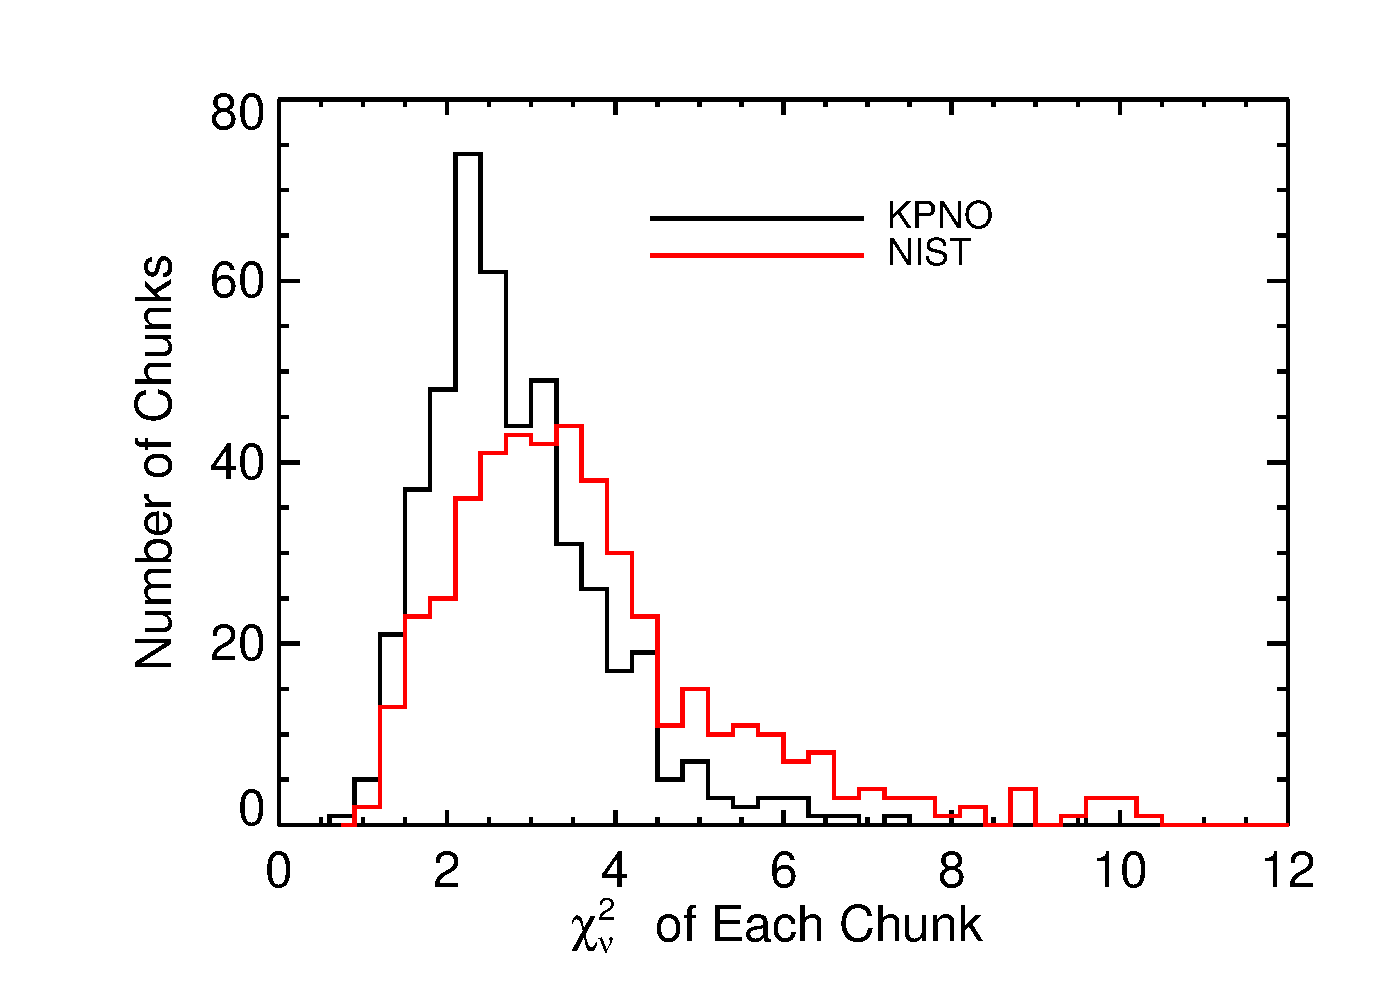
\includegraphics[angle=0.,scale=0.33]{het/hetfts_oldVSnew_chisq.eps}
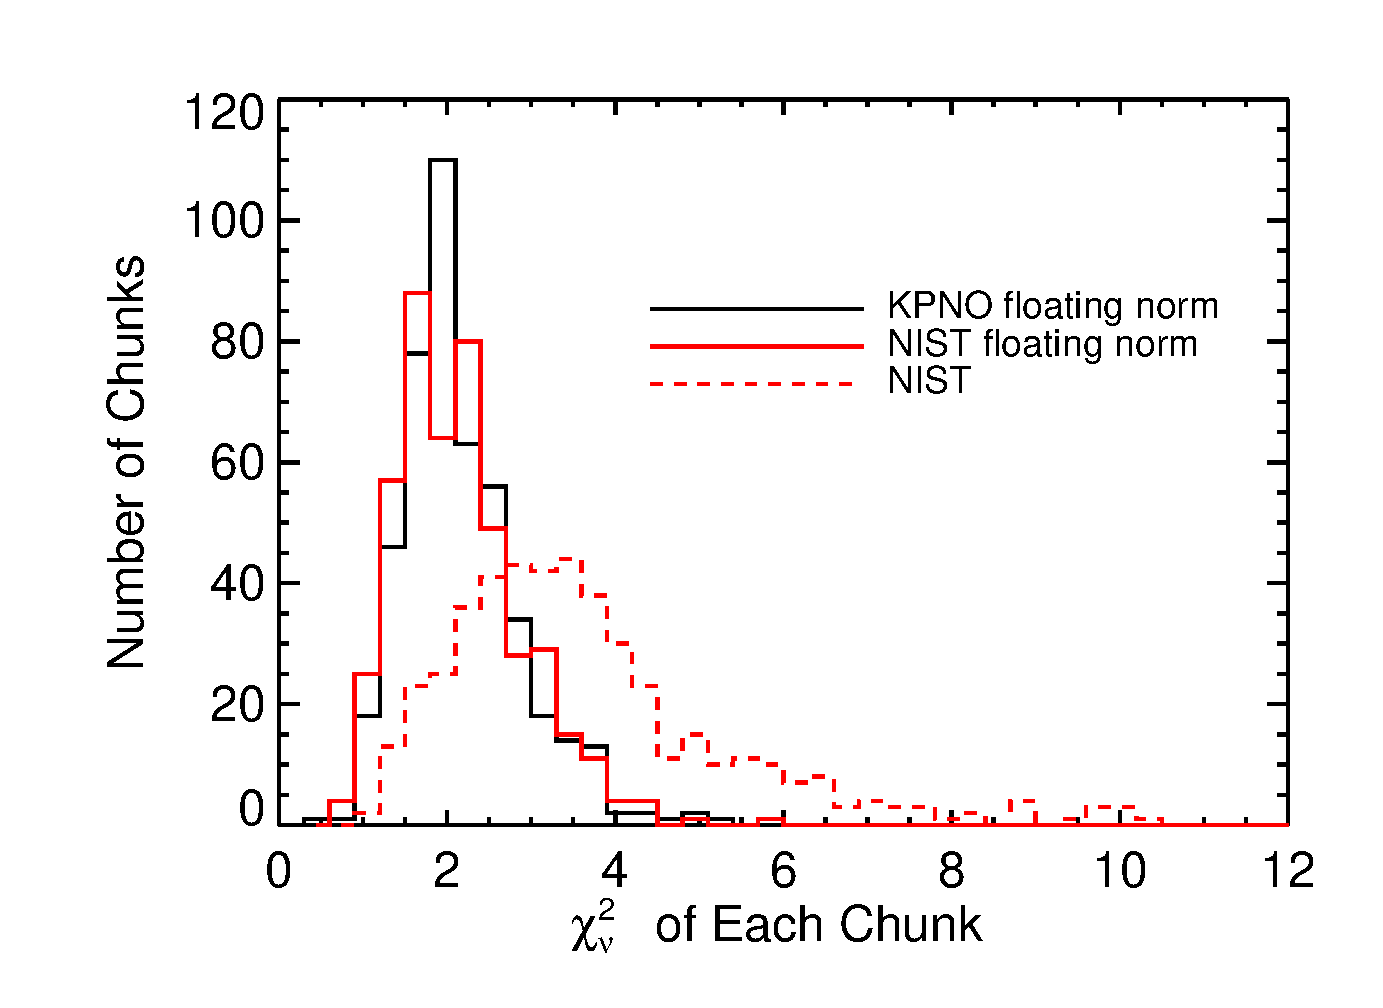
\includegraphics[angle=0.,scale=0.33]{het/hetfts_oldVSnew_chisq_dc.eps}
\caption{Both plots are histograms of \chisq\ values of a single
  iodine observation. Each \chisq\ value in the histogram represents
  the \chisq\ goodness of fit for a $\sim$2\AA\ spectral chunk in this
  iodine observation (each iodine observation is chopped into several
  hundred of chunks and is fitted independently).
%
  \textbf{Left:} \chisq\ histograms for the fit of the iodine
  observation using the KPNO (black) and NIST (red) scan as iodine
  templates, respectively. The KPNO scan obviously performs better.
%
  \textbf{Right:} \chisq\ histograms for the two scans, but both with
  the normalization as a free parameter for each chunk (as we suspect
  the NIST scan has problems in normalization). The two scans now
  perform at essentially the same level. Dashed red line is the same
  red histogram as plotted in the left panel. Notably, the KPNO scan
  also performs better when we float the normalization parameter.
  \label{fig:chisq_old_new}}
\end{figure*}
%----------------------------------------------------------------


Since the direct comparision between the KPNO scan and the NIST scan
has hinted that the `normalization' of the NIST scan might be
problematic, we decide to add a free parameter to account for this
`normalization error' when fitting the iodine observation. The right
panel of Figure~\ref{fig:chisq_old_new} shows the \chisq\ histograms
for the same iodine observation using the two scans, but adding a free
parameter as the `normalization' when fitting each chunk (note: the
normalization parameter is a free parameter for each chunk, not a
global single parameter). The two scans now perform at essentially the
same level.

This is both encouraging and worrisome at the same time. It is
encouraging because it seems that we have found the problem with the
NIST scan, and also have a solution for it. It is very worrisome
because this reveals that:
\begin{itemize}
  \item Even the KPNO cell performs visibly better when we float the
    normalization paramter. This may suggest that there are
    ``normalization'' issues or low frequency errors/noise in the KPNO
    scan as well.
  \item Obtaining high-quality, reliable FTS scans of iodine cell is
    very difficult, and the FTS scans cannot be naively trusted as the
    ``ground truth'' super accurate templates of the complicated iodine
    spectrum.
  \item The reason why adding a ``floating normalization'' fits the
    data better might be because it accounts for optical depths difference
    between the atlas and the actual observations, which may be a result
    of changes in cell temperature or iodine column density in the cell.
  \item The pipeline (when floating normalization as a free parameter)
    cannot distinguish which scan is the ``correct'' one (by \chisq)
    even when two scans differ as much as $\sim$5--10\% at places and
    also have obvious line ratio differneces (see comparison in bottom
    panel of Figure~\ref{fig:fts_old_new}). However, this level of
    difference in FTS may affect the RV precision, and not knowing
    which atlas is the correct one definitely affects our ability to
    search for a better IP and improve the RV precision of \het.
\end{itemize}  

Perhaps even more alarmingly and more puzzling, when we use the KPNO
scan for the iodine cell used at Keck/HIRES to fit an HET/HRS iodine
observation, it yields smaller \chisq\ values than using any of the
other two scans (Figure~\ref{fig:lampi2fit}). The \het\ cell KPNO scan
was taken at the same time using the same FTS machine as the \keck\
cell scan. However, the set-temperatures of these two cells are very
different: the \keck\ cell is designed to work at 50$\degree$C, while
the \het\ cell is designed to work at $70\degree$C.


%----------------------------------------------------------------
% Figure: chisq of iodine observation fit, KPNO HET old scan vs. Keck
% scan
% plots made by
% ~/ExoPlanet-2010-2011/HET-HRS-IP/05-Iodine_FTS_investigation/compare_fts/compare_fts_fits.pro
% stored in ../plots/
\begin{figure}[!th]
\centering
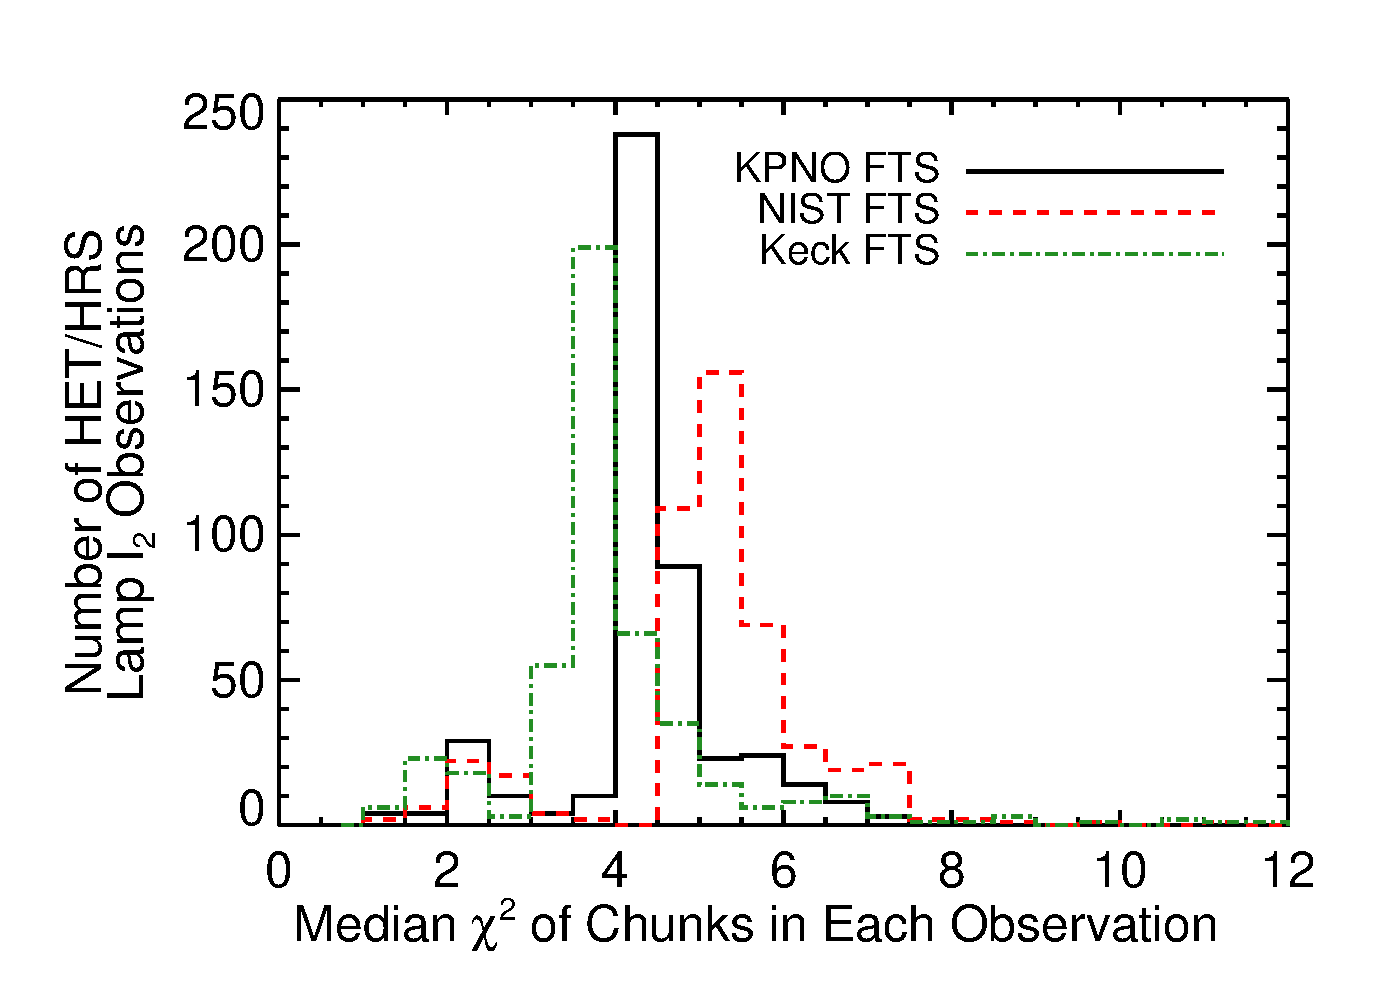
\includegraphics[angle=0.,scale=0.38]{het/het_lamp_i2_fits_kpno_nist_keck.eps}
\caption{Comparison of the median \chisq\ values for fits of iodine
  observations using the \het\ cell KPNO scan (black solid line), the
  NIST scan (red dashed), and the {\em \keck\ cell} KPNO scan (green
  dotted-dashed). Each data point represents the median \chisq\ value
  for all the chunks in a single iodine observation (these are all
  lamp-illuminated -- no B star observation). Results of 550
  \het\ observations are plotted here to illustrate the statistically
  significance. The \keck\ cell KPNO scan provides a better fit than the
  both \het\ scans when fitting \het\ iodine observations.
  \label{fig:lampi2fit}}
\end{figure}
%----------------------------------------------------------------

All of the facts above prompted us to seek a relatively
independent way to perform quality checks for any FTS scan --- not
just comparing their relative qualities or performances. One
natural choice is to obtain spectra taken with high-resolution echelle
spectrographs, which are measurements of the iodine spectrum directly
in the ``real wavelength space'' instead of in the ``Fourier space'', and
thus they serve as good reference spectra as they suffer from
different types of error compared to FTS. Since FTS scans are usually
at a very high spectral resolution ($250,000$--$500,000$), this limits
our choice to essentially only one spectrograph --- the TS12 setting
of the Tull Spectrograph at the 2.7m Telescope at McDonald.


%%%%%%%%%%%%%%%%%%%%%%%%%%%%%%%%%%%%%%%%%%%%%%%%%%%%%%%%%%%%%%%%%%%%%%%%%%%%%%%%%%%%%%%%%%%%%%%%%%%%
\subsection{Methods}

The main purpose of the test using a TS12 spectrum
is to see if it shows significant difference with the KPNO FTS scan,
especially in terms of line depths and ratios. We chose to use the
iodine cell at the Sandiford (2.1m) Telescope, because the HET/HRS
cell was still under active use when we did this test. The Sandiford
cell also has an KPNO FTS scan which was taken together with the KPNO
scan of the HET cell in 1993, so it serves the purpose of testing the
overall quality of the KPNO scans.

We obtained the spectra of the Sandiford iodine cell with TS12 from
September 7 to September 9, 2013, when the telescope was scheduled to
on Cassegrain instrument and the Tull Spectrograph room was free for
use. The description on data acquisition and reduction in this section
and the results presented in the next section are for the the
contiguous $\sim$30\AA\ spectrum region that we took on the second and
third day of observation.

\textbf{\textit{Hardware Settings:}} We used the TS12 arm of the Tull
Spectrograph, and the specific instrument choices are listed in
Table~\ref{tab:hardware}. The cell was kept at a temperature of
49.9--50.1$^\circ$C, the same as its working temperature for RV work
and its temperature when the KPNO was taken (50$^\circ$C). Slit \#23
is chosen to maximize SNR while maintaining sufficient resolution ---
it is among the longest slit and is also the second narrowest slit.

%----------------------------------------------------------------
% Table: variability analysis results
\renewcommand{\arraystretch}{1.3} % more row spacing for the table
\begin{deluxetable}{rl}
%\rotate
\tabletypesize{\scriptsize}
\tablewidth{180pt}
\tablecaption{Hardware Settings for TS12 Iodine Spectrum Test\label{tab:hardware}}
\startdata
  \hline
  \multicolumn{2}{c}{Tull Spectrograph, TS12, Coude107} \\
  \hline
  Echelle & E1 \\
  Cross Disperser & c \\
  CCD & TK4, 1024$\times$1056 \\
  On-chip Binning & 1$\times$1 \\
  Slit & \#23 (L$\times$W $=30\arcsec \times 0\arcsec .32$)
\enddata
\end{deluxetable}
%----------------------------------------------------------------


\textbf{\textit{Observation:}} A single exposure frame for the iodine
spectrum covers about 1.9\AA. The dispersion direction runs vertically
along the chip with increasing wavelength when increasing the $y$-axis
pixel. The dispersion scale is about 0.002\AA\ per pixel ($\sim$7
pixels per resolution element). We immediately preceded or followed
each exposure with a flat fielding frame. The exposure times for the
iodine and flat frames are both 45 seconds to achieve a
signal-to-noise ratio (SNR) of 160 per pixel. Neighboring frames
differ by about 1\AA\ in absolute wavelength. If prominent Solar or
ThAr line was predicted within the wavelength coverage of a frame,
then we also took a Solar or ThAr frame to verify the rough wavelength
solution (the exposure time varied --- typically a couple minutes to
up to 10 minutes). We took dark frames (45s each, about 10 frames) in
the morning at the beginning of each day.

\textbf{\textit{Reduction:}} We combined and averaged all available
dark frames and created a master dark frame. Then we subtracted the
master dark from all flat and iodine frames. After outlier rejection
(cosmic rays, chip defects, etc.), we modeled the scattered light for
each row of pixels by using the region outside the slit image.  We
stacked 160 neighboring rows and fitted a third order polynomial along
the column, and then interpolated for the amount of scattered light
within the slit image region and subtracted it. Both the flat and
iodine frames have scattered light removed. We then normalized the
flat frames and divided each iodine frame by its associated normalized
flat (for the slit image regions only).

\textbf{\textit{Extraction:}} As the slit does not lie perfectly along
the $x$-axis direction on the chip, we corrected for this by cutting
columns along the dispersion direction and cross-correlating the
columns. Then we interpolated and shifted the columns to create an
aligned image, which we stacked along the $x$-axis direction and
obtained the reduced, extracted spectrum. Each spectrum is then
normalized by dividing the estimated continuum (top 5\% counts). Due
to lower quality of scattered light removal near the edge of the chip,
we discarded the top 80 and bottom 80 rows of pixels. Thus the
extracted spectrum from each frame is about 1.6\AA\ across (instead of
1.9\AA). The $\sim$20 frames are then `stitched' together by finding
the overlapping region through cross correlation for each pair of
neighboring frames and taking into account the changes and differences
of dispersion scales across frames.
\begin{comment}
For the overlapping region, the spectrum in the bluer frame is
`projected' onto the redder frame by taking into account the changes
and differences in pixel dispersion scales in the two frames. The
overlapping spectral region in the stitched spectrum thus has the
dispersion scale of the redder frame, but it preserves the
normalization of the bluer frame. This way the two frames are stitched
together.
\end{comment}

\textbf{\textit{Mapping onto FTS:}} To compare with the KPNO FTS
spectrum, we chopped the TS12 spectrum into 2\AA\ chunks and project
each chunk onto the FTS spectrum by cross correlation. In this way we
obtained the absolute wavelength solution and dispersion scale (as set
by the wavelength solution of the FTS scan) for the TS12 spectrum. The
results of comparison are shown in the next section.



%%%%%%%%%%%%%%%%%%%%%%%%%%%%%%%%%%%%%%%%%%%%%%%%%%%%%%%%%%%%%%%%%%%%%%%%%%%%%%%%%%%%%%%%%%%%%%%%%%%%
\subsection{Results}

%----------------------------------------------------------------
% Figure: TS12 spectrum vs. KPNO FTS scan, native resolution, selected
% 2A chunk
\begin{figure*}[!th]
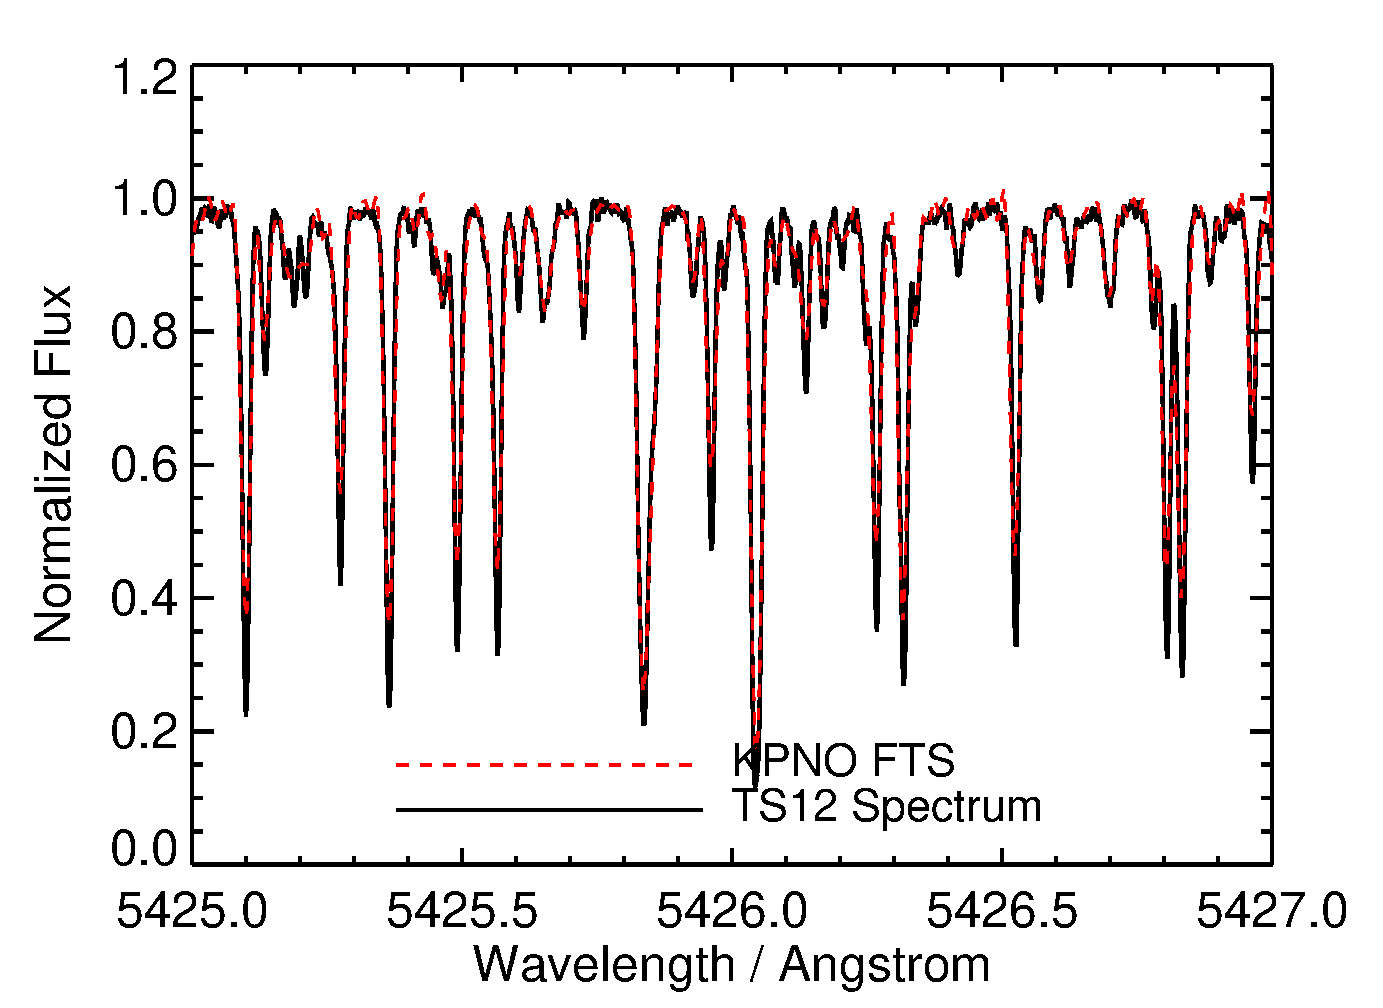
\includegraphics[angle=0.,scale=0.33]{het/chunk_5425A_original_sclrem.eps}
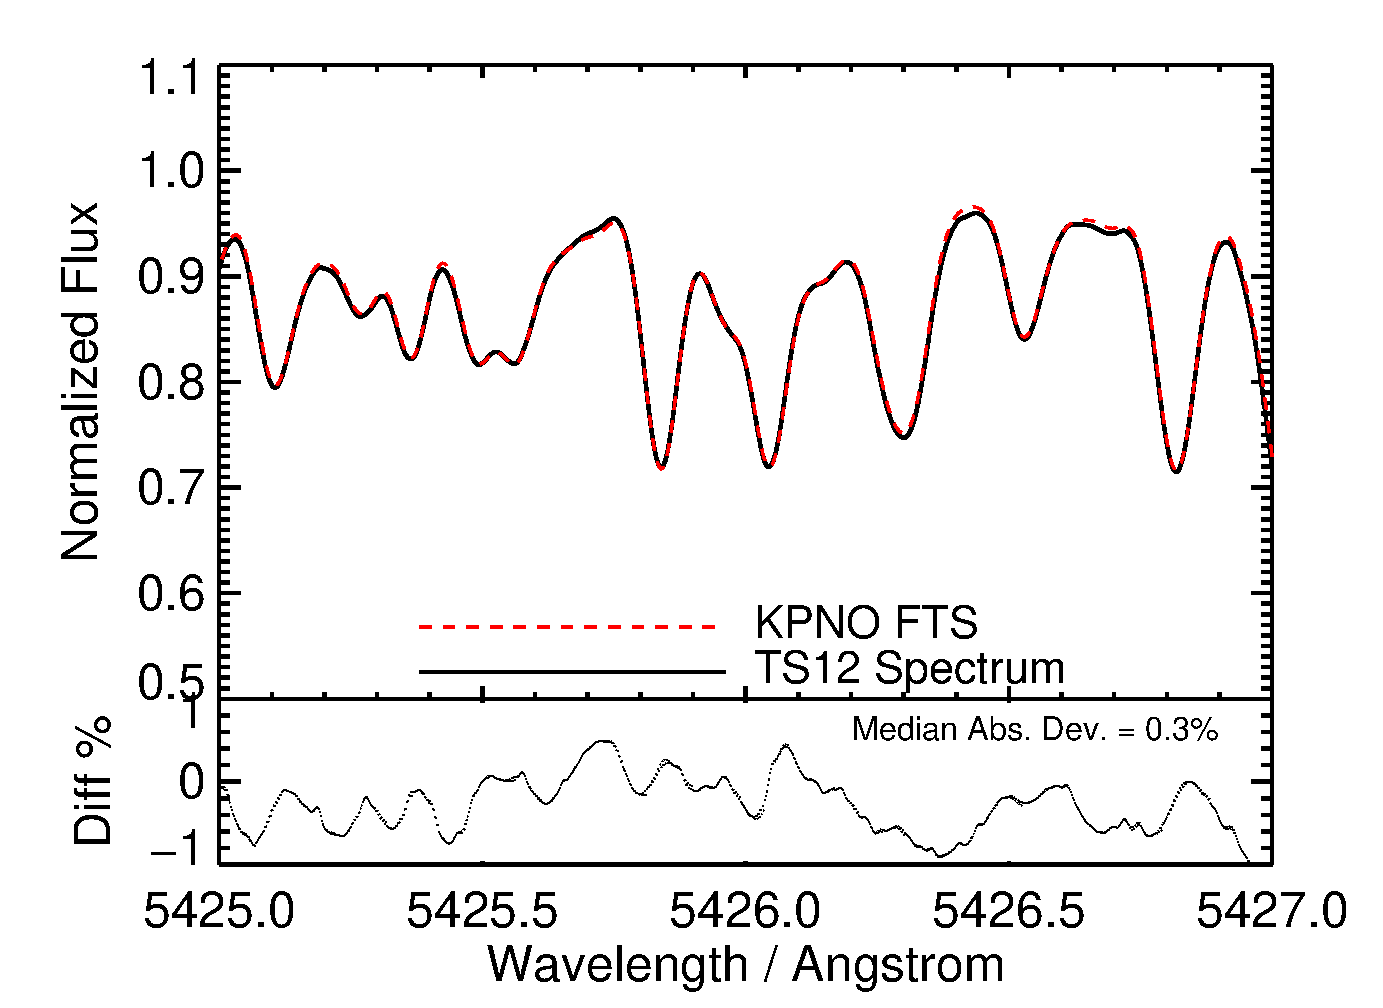
\includegraphics[angle=0.,scale=0.33]{het/chunk_5425A_60k_gaus_sclrem_diff.eps}
\caption{Comparison of the Sandiford iodine cell KPNO FTS spectrum and
  the spectrum taken with TS12. \textbf{Left:} Comparison of the two
  spectra in their native resolutions (both about
  $450,000$--$500,000$). \textbf{Right:} Comparison of the two spectra
  convolved down to about $60,000$ resolution, which is the resolution
  of typical iodine observations or radial velocity observations
  (star$+$iodine). Bottom panel shows the residuals in percentage of
  the TS12 spectrum minus the KPNO spectrum, with a median absolute
  deviation of 0.3\%.
  \label{fig:ts12}}
\end{figure*}
%----------------------------------------------------------------

The left panel of Figure~\ref{fig:ts12} shows a direct comparison of the reduced
TS12 spectrum (a random 2\AA\ chunk) with the KPNO FTS scan, at their
native resolutions. Note that the TS12 spectrum appears to have a
higher resolution than the FTS scan. According to the header of the
FTS scan, its resolution is about $491,000$. An FFT analysis on the TS12
spectrum (to see where the high-frequency signal cuts off and becomes
indistinguishable from the noise) shows that its resolution is about
$455,000$ and maybe even higher.


%----------------------------------------------------------------
% Figure: TS12 spectrum vs. KPNO FTS scan, 60k, all, with residuals
\begin{figure}[!th]
\centering
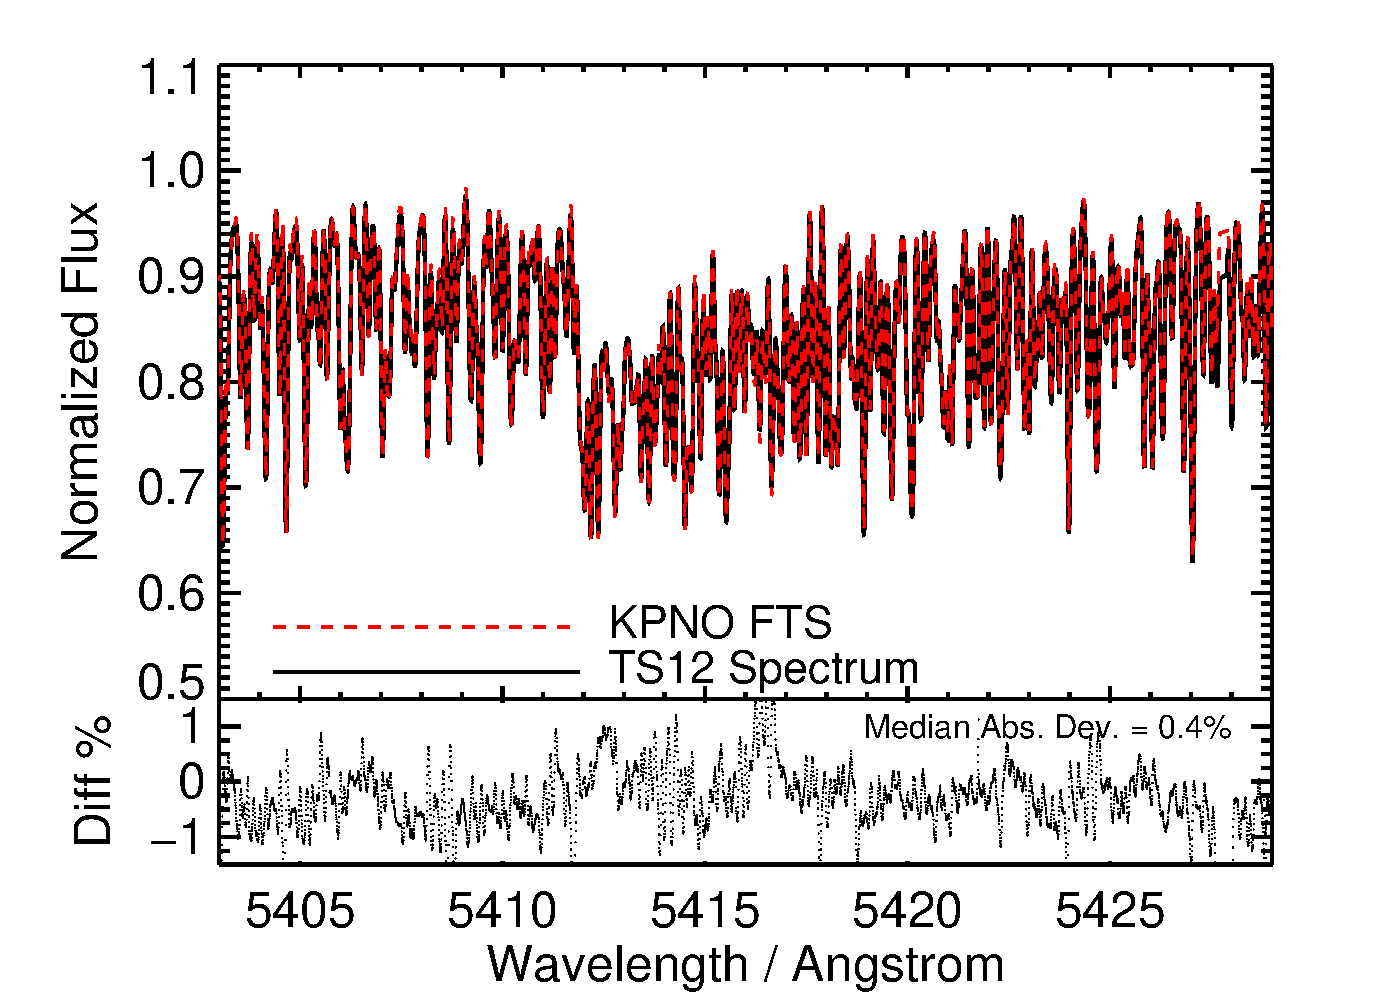
\includegraphics[angle=0.,scale=0.45]{het/all_60k_gaus_sclrem_diff.eps}
\caption{The same as the right panel of Figure~\ref{fig:ts12}, the
  KPNO spectrum and the TS12 spectrum both at $60,000$, but for the entire
  $\sim$30\AA\ TS12 spectrum available. 
  \label{fig:60k_all}}
\end{figure}
%----------------------------------------------------------------


To make a more direct comparison and also to see the differences of
the two spectra (if any) would make a significant impact when fitting
a $60,000$ resolution iodine observation, we degraded the resolution
of both spectra to $60,000$ by convolving them with a Gaussian of a
proper width. We analyzed the FFT spectra of the two convolved spectra
to make sure that they are indeed at the same resolution, and both are
around $60,000$. The right panel of Figure~\ref{fig:ts12} illustrates
the comparison of the two spectra at $R\sim60,000$, with residuals of
the TS12 spectrum minus the KPNO FTS spectrum plotted in the bottom
panel. The two spectra differ by a median absolute deviation of 0.3\%
($0.4\%$ for the entire $\sim$30\AA\ spectrum available as shown in
Figure~\ref{fig:60k_all}). As the TS12 spectrum has a SNR of about 160
and we have convolved the comparison spectrum down to $R\sim60,000$,
the expected shot noise should be $\sim 1/160\times
\sqrt{450,000/60,000}=0.23\%$. The additional $\sim 0.1\%$--$0.2\%$ of
noise may come from flat fielding, scattered light removal, cosmic ray
removal and interpolation between pixels, stitching of spectra,
projection onto the FTS spectrum and interpolation for comparison
purposes, and so on.

For comparison: when fitting the HET/HRS Iodine observation used for
creating Figure~\ref{fig:chisq_old_new} (median SNR for a typical
chunk is $\sim$150, or 0.65\% shot noise), for a typical chunk, the
median absolute deviation between the observation and the best-fit
model is 0.73\% (the rms value is 1\%, thus \chisq\ is $\sim 2$--$3$).


% SUMMARY
\textbf{\textit{Conclusion:} Through this test, we have demonstrated that an
  iodine cell spectrum taken with TS12 has the same quality as an FTS
  scan to serve as the `true solution' of the iodine spectrum (caveat:
  lack of wavelength solution). A comparison between the TS12 spectrum
  and the FTS scan of the same cell serves as a good method to check
  the quality of FTS scans.}



ZZZ paragraphs on temperature change from NESSF renewal, needs heavy modification


A ``ground truth" iodine atlas is crucial for the precise iodine
radial velocimetry. It is used for modeling the observed iodine lines
in the stellar$+$iodine RV observation to anchor the absolute
wavelengths and the spectrograph response function. Such a ``ground
truth" atlas is normally obtained through a Fourier Transform
Spectrometer (FTS). Our previous work has revealed potential problems
with FTS atlases, and in our original proposal, we promised to use the
TS12 arm of the Tull spectrograph at McDonald Observatory to validate
the qualities of the FTS iodine atlases for HET/HRS, MINERVA, and the
McDonald 2.7m.

In October 2014, the TS12 observations were successfully carried
out. All data are reduced and we have made comparisons between the
TS12 spectra and FTS scans. For the 2.7m cell, its TS12 spectrum
matches very well to its FTS atlas, again (together with the 2.1m cell
data from 2013) proving that TS12 is an appropriate tool for
validating FTS atlases. The TS12 spectra for the MINERVA cell is also
ready, and right now we are waiting for the FTS expert on our team to
reduce the MINERVA FTS data for comparison, which is expected to be
done before June (first light of the proto-type MINERVA spectrograph).

Finally, for the HET/HRS iodine cell, we have taken its TS12 spectra
at three different temperatures (50, 60, and 70$\degree$C; the RV
working temperature for the cell is 70$\degree$C). Our main findings
(both are first-time discoveries for iodine RV work) are as follows:

(a) Temperature change (5--10$\degree$C) in iodine cell matters: The
long suspected temperature-induced iodine spectrum change was finally
confirmed, which is seen very visibly among the TS12 spectra taken at
three different temperatures. Based on our NIST FTS atlases taken at
two different temperatures, temperature change on the order of
10$\degree$C should not induce visible line changes. However, we
suspected issues with temperature control and data calibration with
the NIST atlases, and the TS12 spectra confirmed our suspicion and
proved that temperature on the order of even 5$\degree$C would have
manifested as significant line changes (for precise RV purposes).

(b) The HET/HRS cell very likely has changed over time: The TS12
spectra match better with the more recent but potentially problematic
NIST FTS atlas, which had worse $\chi^2_\nu$ fit than the old KPNO
atlas. This is completely unexpected and suggests that: the NIST atlas
was perhaps taken at the correct temperature (i.e.\ the KPNO atlas was
at a lower and wrong temperature) but the worse fit was caused by
calibration errors in the atlas; and/or the temperature or optical
depth of the cell changes over the course of 20 years, and hence the
differences between these three spectra (Figure~\ref{het:fig:hetts12}); and
further more, it is possible that the temperature/optical depth of the
cell changes on a much shorter scale during the observing seasons, and
most of the time it stays at a temperature/optical depth that is
similar to the one when the KPNO atlas was taken (e.g.\ actually at a
lower temperature though thought to be at 70$\degree$C).



%----------------------------------------------------------------
% HET/HRS cell, TS12 vs KPNO vs NIST
% plot from ~/TS12/match_fts/figure/, made by plotcomp.pro
% grabbed from ~/ExoPlanet-2010-2011/Professional_Development/201402-NESSF/renewal/proposal/
\begin{figure}
\centering
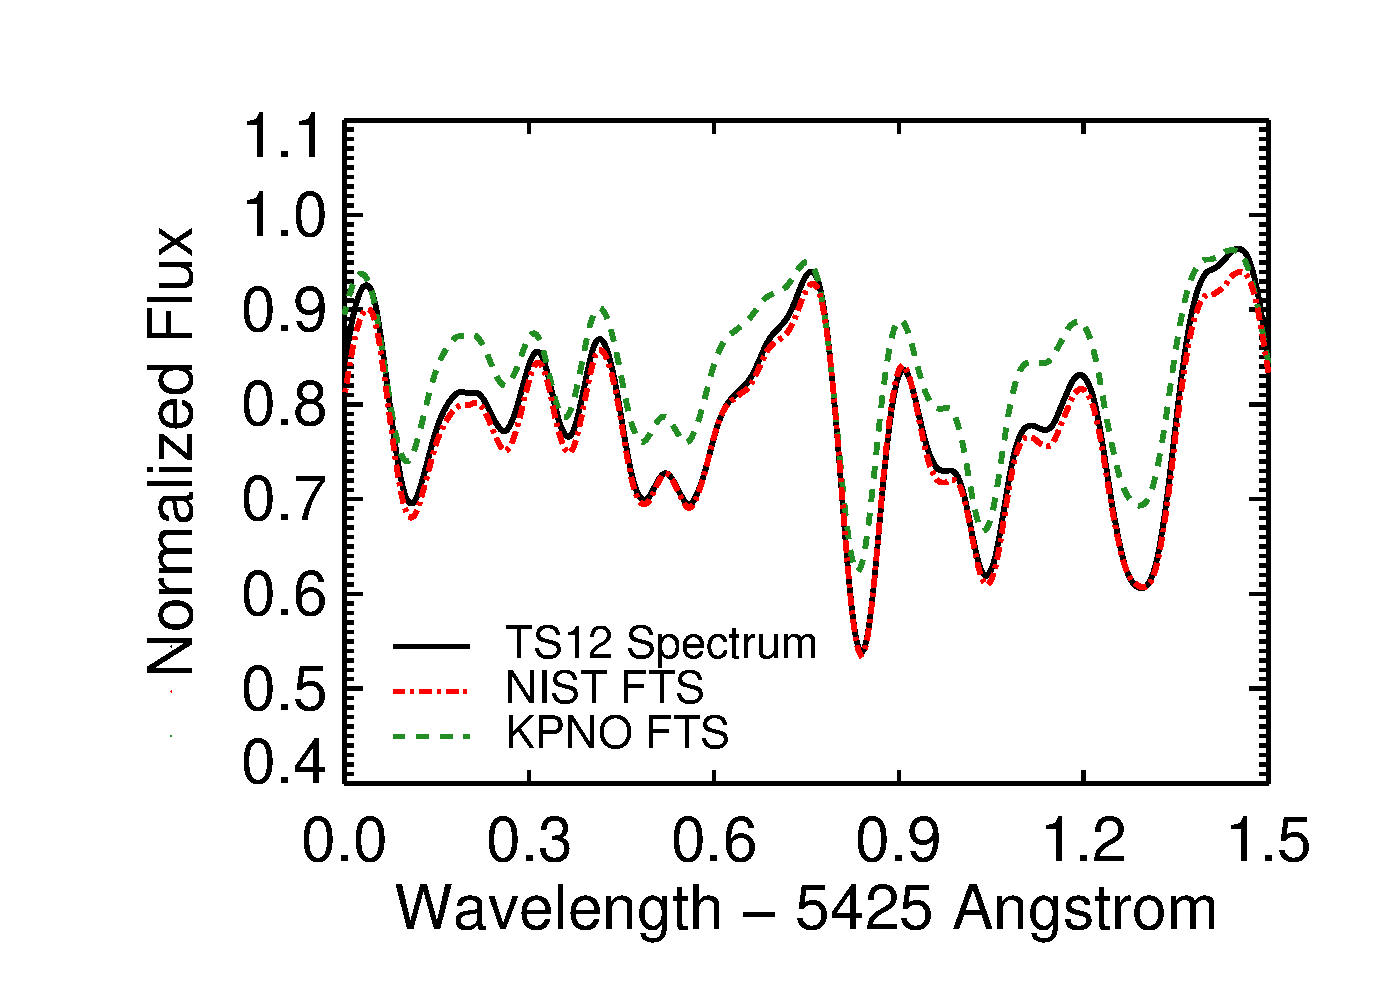
\includegraphics[scale=0.5]{het/het70_comp.eps}
\caption{TS12 spectrum (black solid line) vs.\ NIST FTS (red
  dotted-dashed) vs.\ KPNO FTS (green dashed) for the \het\ iodine
  cell at 70$\degree$C, all convolved down to a resolution of R $=$
  60k (the same as a typical \het\ observation) for comparison
  purposes. The TS12 spectrum matches the NIST FTS better, having
  deeper lines compared to the original KPNO FTS. The remaining
  difference between NIST FTS and the TS12 spectrum might be due to
  differences in cell temperatures or other changes with the cell. 
\label{het:fig:hetts12}}
\end{figure}
%----------------------------------------------------------------



To answer these questions and to actually resolve the issue of a
changing cell, we have found a possible third venue that might provide
reliable, ultra-high resolution, and wavelength calibrated iodine
atlas -- a theoretical code that computes iodine transmission spectrum
(at any specified temperature) based on both physics and empirical
calibrations (IodineSpec5; \citealt{iodinespec5}). We have
successfully installed and learned the code, and properly translated
the code output into practical astrophysical units and to account for
optical depth differences. Figure~\ref{het:fig:iodspec5} shows the results.





%----------------------------------------------------------------
% HET/HRS cell, IodineSpec5 2 temperatures vs. NIST, and KPNO
% plot from ~/ExoPlanet-2010-2011/IodineSpec5/, made by plots_general.pro
\begin{figure}
\centering
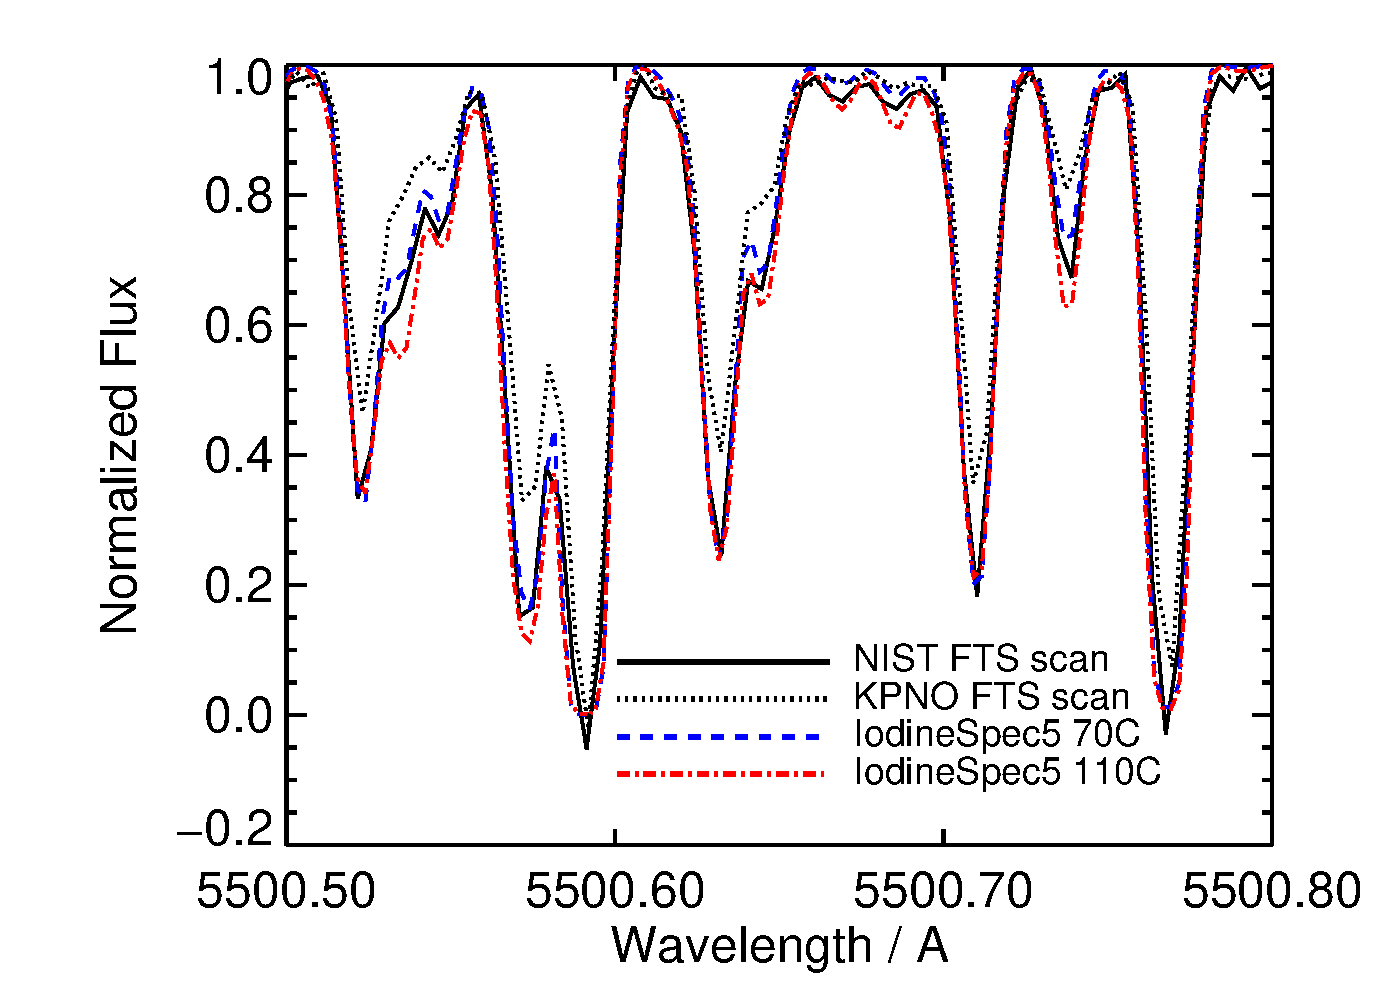
\includegraphics[scale=0.5]{het/HET_NIST_temp.eps}
\caption{NIST FTS (black solid lines) and KPNO FTS (black dotted
  lines) compared with theoretically computed iodine lines at
  70$\degree$C (blue dashed) and 150$\degree$C (red
  dotted-dashed). There are two free parameters for the theoretical
  lines: temperature and iodine column density. For this plot, we optimized
  the iodien column density for the theoretical lines at both
  temperatures to try to fit the NIST FTS. As illustrated, neither
  temperature can produce a good fit, and the best-fit temperature is
  around 110$\degree$C. Note that the theoretical lines and the NIST
  FTS have different broadening kernels. The NIST and KPNO FTS scans
  probably differ in both optical depth and cell temperature.
\label{het:fig:iodspec5}}
\end{figure}
%----------------------------------------------------------------


%----------------------------------------------------------------
% NIST scan fit by IodineSpec5 and comparison with FTS
% plot made by
% ~/ExoPlanet-2010-2011/HET-HRS-IP/05-Iodine_FTS_investigation/compare_fts/fit_temp_change.pro and saved therein
\begin{figure}
\centering
\subfloat{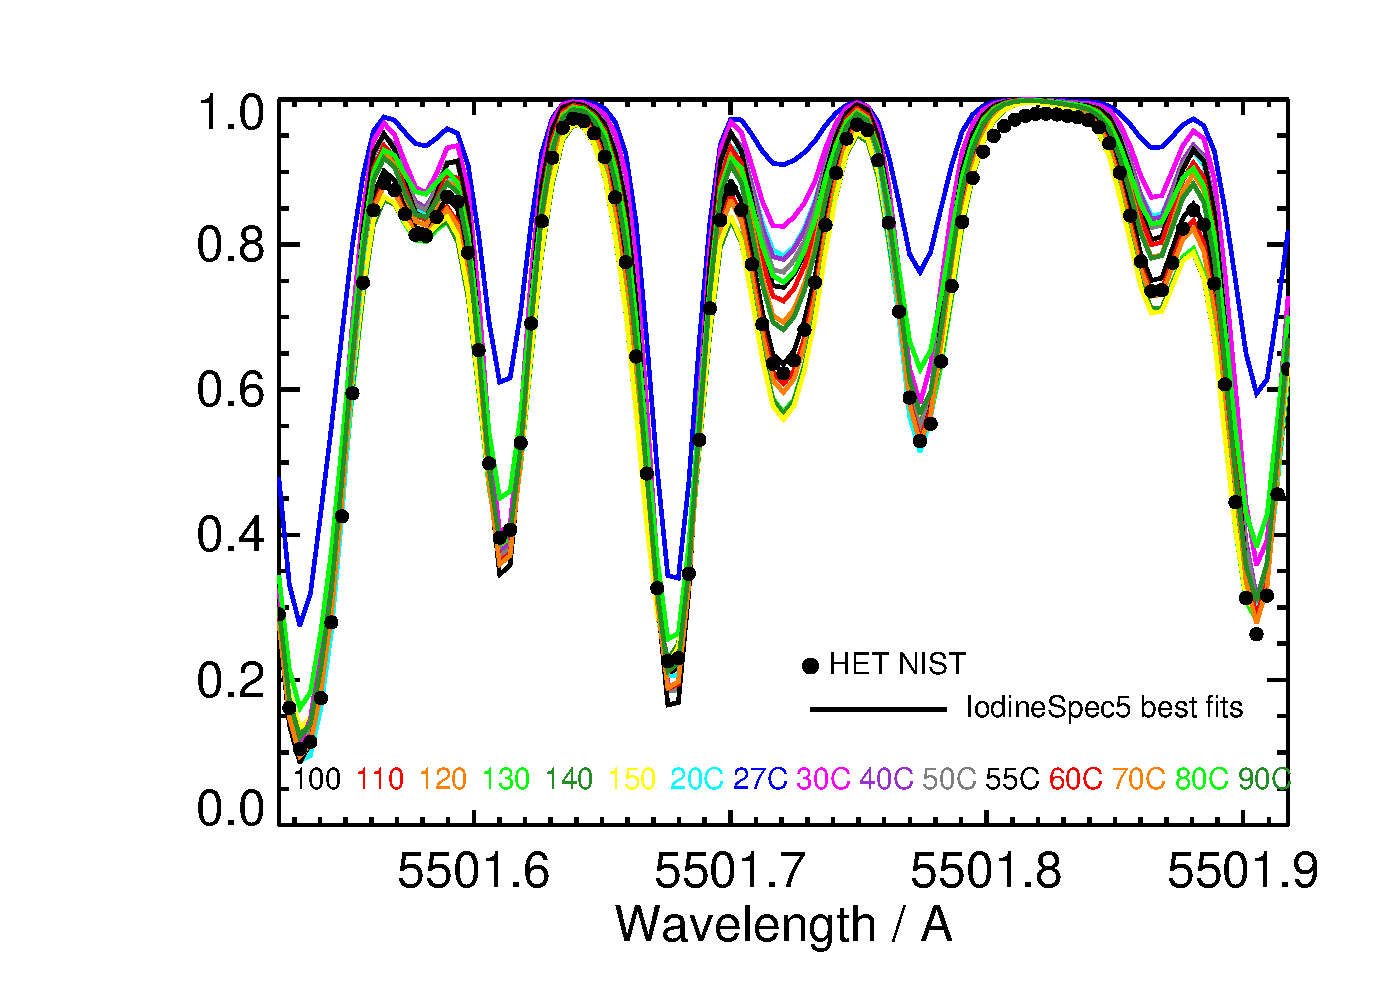
\includegraphics[scale=0.5]{het/hetnist_bestfits.eps}}\
\subfloat{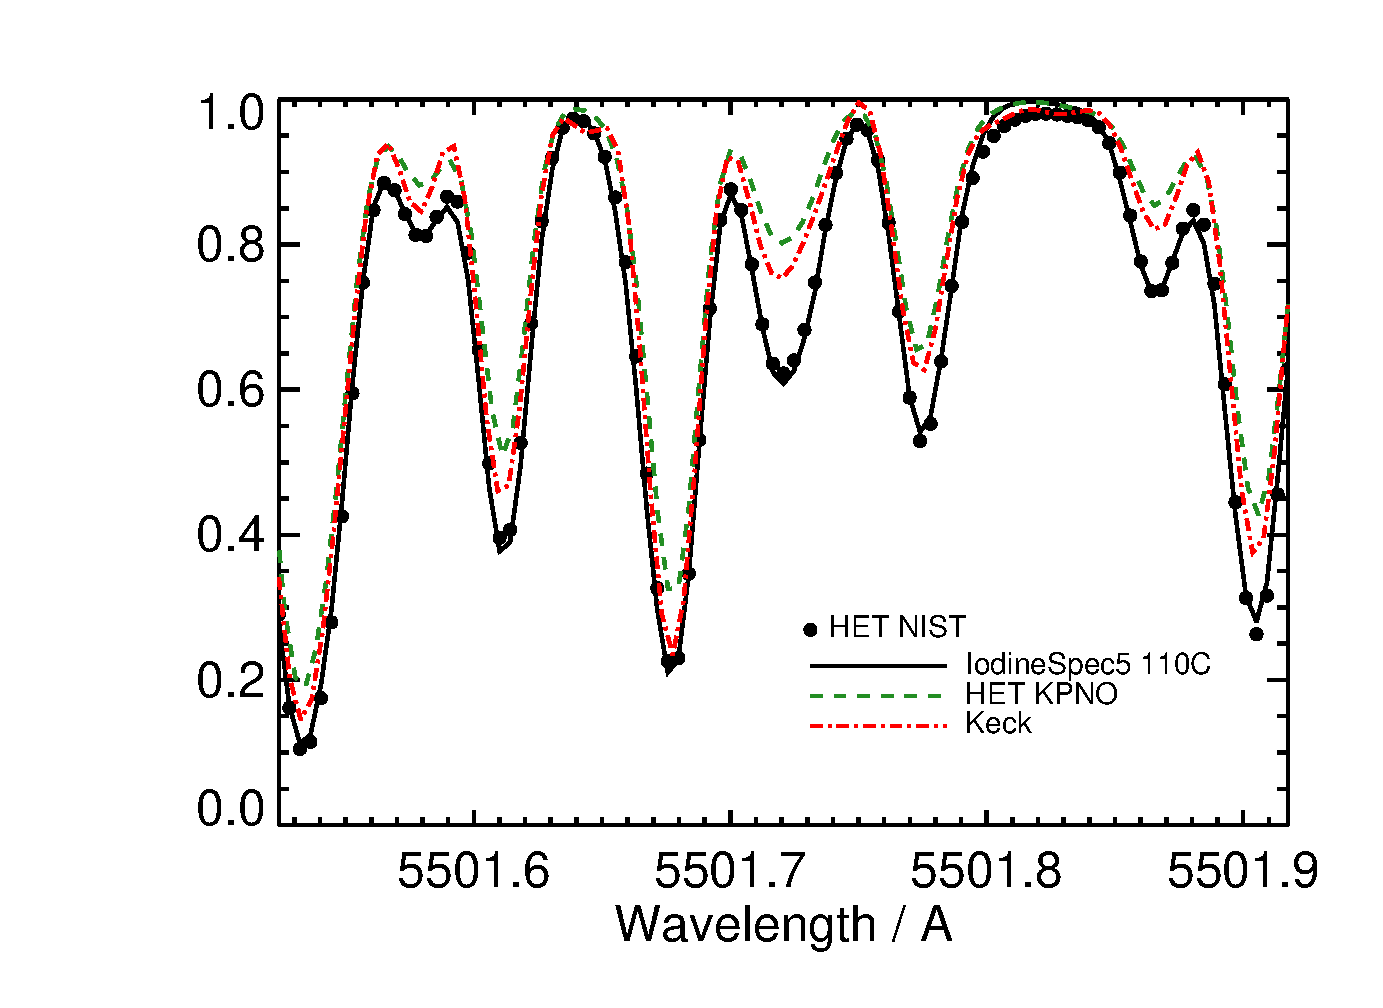
\includegraphics[scale=0.5]{het/hetnist_compWithOthers.eps}}
\caption{{\bf Top:} Fitting \het\ NIST scan (black dots; temperature
set at 70$\degree$C) with IodineSpec5 synthetic iodine lines at
various temperatures and column densities. {\bf Bottom:} The \het\
NIST scan (black dots) overplotted with the best-fit IodineSpec5 model
(black solid line; at 110$\degree$C) and the \het\ cell and \keck\ 
cell KPNO scans. All spectra in both panels are convolved down to a
resolution of 150,000 (roughly \keck\ KPNO FTS scan resolution) to
wash out the intrinsic IP difference between FTS scan (sinc function
IP) and the synthetic spectrum (only natural broadening IP models).
\label{het:fig:nistfit}}
\end{figure}
%----------------------------------------------------------------


%----------------------------------------------------------------
% TS12 fit by IodineSpec5 and comparison with FTS
% plot made by
% ~/ExoPlanet-2010-2011/HET-HRS-IP/05-Iodine_FTS_investigation/compare_fts/fit_temp_change.pro and saved therein
\begin{figure}
\centering
\subfloat{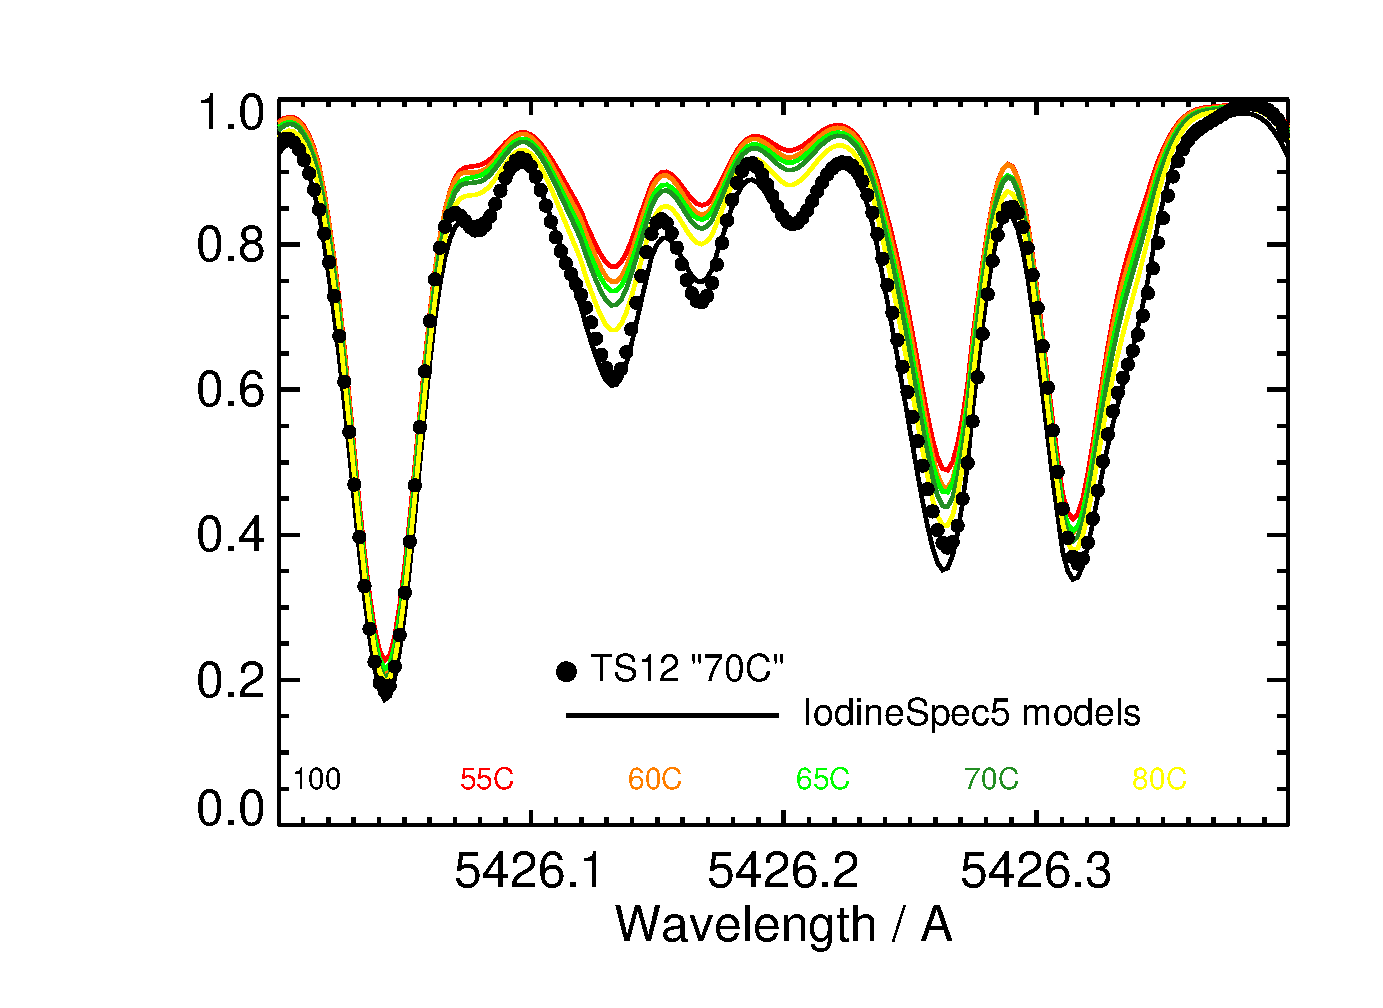
\includegraphics[scale=0.5]{het/ts12_70_bestfits.eps}}\
\subfloat{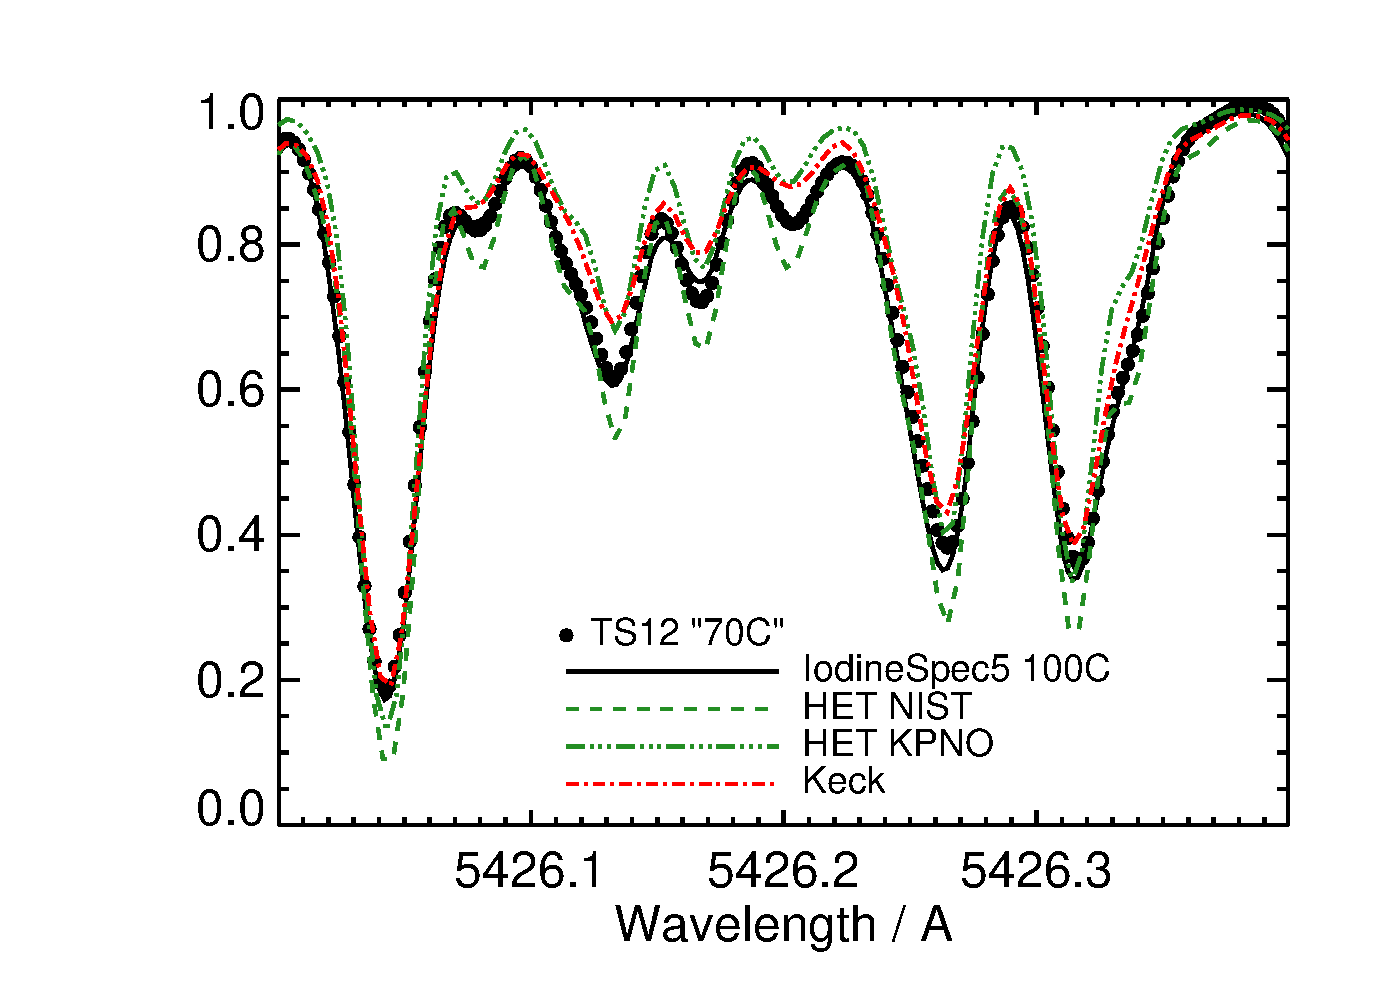
\includegraphics[scale=0.5]{het/ts12_70_compWithFTS.eps}}
\caption{{\bf Top:} Fitting the TS12 spectrum (temperature set at
70$\degree$C; black dots) with IodineSpec5 models, with fixed column
density derived from best fits using \het\ KPNO and NIST scans. {\bf
Bottom:} The best-fit temperature for the TS12 spectrum is about
100$\degree$C (black solid). It is clearly at a lower temperature than
the NIST scan (green dashed) but at a higher one than the KPNO one
(green dotted-dashed). Again, all spectra in both panels are convolved
down to $R=$ 150,000.
\label{het:fig:ts12fit}}
\end{figure}
%----------------------------------------------------------------
